\documentclass[12pt,a4paper,oneside,titlepage]{article}
%titlepage prints the title on it's own page in article class

%doublespace my text
\renewcommand{\baselinestretch}{1.5}

%reduce the hyphenation of words
\sloppy

%prints a small space between paragraphs and removes the indenting of the first line
\setlength{\parskip}{2ex plus0.5ex minus 0.2ex}
\setlength{\parindent}{0em}

%csquotes - provides multilingual quoting - keeps babel happy
\usepackage{csquotes}
%babel required for biblatex to work. Specifying british last make it the language in use
%\usepackage[english,british]{babel}
\usepackage[british]{babel}

\usepackage[style=authoryear,backend=biber,
	giveninits=true,
	uniquename=init,
	language=british]{biblatex}

\usepackage{graphicx}

\defbibnote{needsfixing}{\emph{(this formatting needs looking at -- not currently to LSBU standards.
For example, need to include names of all the authors.)}}
% Add my bibliography file here
\addbibresource{references.bib}

%rotating allows text to be printed sideways
%multirow allows tables with cells spanning more than one row
% Remove this if not required
%\usepackage{rotating,multirow}


\begin{document}
\author{Gregory Cartwright}
\title{}
%\maketitle
\section*{Introduction}

\subsection*{Context}
The author is an advanced nurse practitioner (ANP) in a community Trust.
The Trust has community hospitals which have wards for inpatient rehabilitation and
medical stepdown. Their are 12 wards accross 8 community hospitals. Each ward has
an ANP who works on the ward to provide medical management of the patients during 
the hours of Monday to Friday, 0900 to 1730. Outside of these hours, medical care 
is provided by the out of hours GP service. 

Most patients are admitted to the community hospital wards for either rehabilitation
or medical stepdown. The majority of these patients come following an acute admission
where they have been stabilised medically but are often deconditioned as a result
of acute illness and are not ready to go home. At this stage their needs include 
ongoing medcial treatment and monitoring and further assessments and treament such 
as physiotherapy and occupational therapy to prepare them for discharge home.

Some patients are admitted directly from home because they have medical or rehabilitation
needs that cannot be met at home but do not require an admission to an acute setting.
A minority of patients are admitted for paliative care.

When patients are admitted to one of these wards they have a comprehensive geriatric 
assessment (CGA) \parencite{bgs:14} performed by the multi-disciplinary team (MDT).
An international meta-analysis found that, when compared with general medical care,
CGA was effective at keeping older people alive and living in their own homes at
twelve months post admission with a number needed to treat of 33 \parencite{ellis:11}.

\subsection*{Frailty}
Frailty is widely agreed to be a condition where the maintenance of homeostasis 
becomes vulnerable to 
small stressors \parencite{vellas:16} and is acknowledged to be a large problem amongst the ageing population 
\parencite{clegg:13}. Examples of such stressors include changes in environment and minor
illness. The consequences of exposure to these include delirium, significant reduction in mobility,
falls, increased dependency, non-specifc failure to thrive and death 
\parencite{bgs:14,vellas:16,oliver:14}.

\subsubsection*{Prevalance}
Frailty is common amongst older people, specifically those who are housebound or 
have care at home or live in a care home \parencite{oliver:14}. An international systematic review found 
that at least 10\% of people aged over 65 had frailty and of those aged 85 or over
at least 26\% were frail \parencite{collard:12}. There are various methods and tools used to assess frailty.
Some of these count the number of deficits from a particular set that a person has. 
\textcite{sternberg:08} suggest that such a tool is not practical for use in a clinical
setting, being more suitable to assessing populations for strategic planning. 
Other tools require numerous specific measurements to be taken, again making them
less suitable for clinical use \parencite{martin:08} and possibly more suited to research purposes
\parencite{ensrud:08}. \textcite{romero-ortuno:16} argue that this fragmentation should not
be viewed as a problem as each frailty assessment tool is suited to a different 
purpose. 

In both the clincal area which the author works and the emergency department at
the local acute Trust, frailty is assessed using the Clinical Frailty Scale (CFS).
See appendix~\ref{appendix:CFS}.
The CFS is a tool that has been validated for use in cinical practice 
\parencite{rockwood:05}. It rates frailty based on the person's level of independence
and dependence, giving them an ordinal postion on the continuum from very fit and completely 
independent, CFS of 1, to very severely frail and completely dependent, CFS of 8.
There is also a CFS of 9 for those who are terminally ill. The CFS is based on clinical
judgment of the patient and is therefore suited to clinical use, certainly after
the patient has had a CGA \parencite{bgs:14}.

The CFS score has recently bee introduced to the community hospital wards and the
score is not being used for any specific purpose, it is hust being entered into 
the patients' notes for people to refer to. These scores are not being collected, 
but the author suspects that the proportion of inpatients who are at least 
moderately frail, with CFS at least 6, will be quite high. Specifically because
CFS is partly based on a person's ability to carry out activities of daily living (ADLs)
and instumental activities of daily living (IADLs) and one reason that many patients
are admitted to the community hospital is that they need rehabilitation to be
able to carry out ADLs and IADLs. Indeed in a study to assess the prevalence of frailty
in France, \textcite{cossec:16} found that dependency on others for IADLs was an 
independent determinant of frailty.

\subsubsection*{Consequences of frailty}

By definition, frailty is a state where a small change, intrisic or extrinsic, can
lead to multiple consequences \parencite{collard:12}. These can be severe, including 
death. An examination
of all bereavements of adults in England that were not due to accident, homicide or suicide for 
a four month period in 2012 was 
carried out \parencite{ons:13}. It found that the proportion of deaths
that were not due to cancer or any cardiovascular disease was 42\%. In the over 80
age group this was 80\%. The most recent edition of this survey from 2015 found
that the overall proportion of non-cancer and non-CVD deaths was slightly higher 
at 46\% \parencite{ons:16}, but did not provide a breakdown by age group.

How many of these deaths were due to frailty is not know, however 
a Canadian study that examined all deaths in Alberta found that frailty was the
cause of 30\% of mortality \parencite{fassbender:09}.

\subsubsection*{Interventions for frailty}

\clearpage
\printbibliography[prenote=needsfixing]

\clearpage
\begin{appendix}
\section{Clinical Frailty Scale}
\label{appendix:CFS}
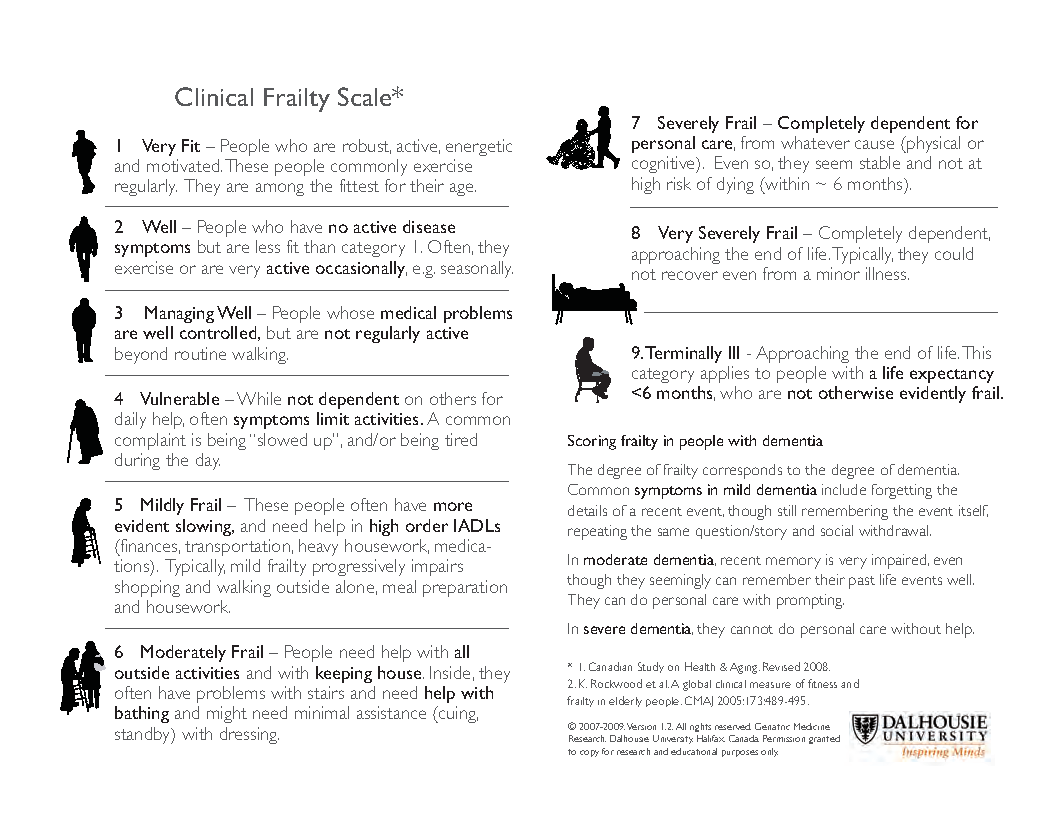
\includegraphics[width=\textwidth]{CFS}
\end{appendix}

\end{document}
